\section{Derivatives of Inverse Functions}\label{sec:deriv_inverse_function}

%Recall that a function $y=f(x)$ is said to be \textit{one-to-one} if it passes the horizontal line test; that is, for two different $x$ values $x_1$ and $x_2$, we do \textit{not} have $f(x_1)=f(x_2)$. In some cases the domain of $f$ must be restricted so that it is one-to-one. For instance, consider $f(x)=x^2$. Clearly, $f(-1)= f(1)$, so $f$ is not one-to-one on its regular domain, but by restricting $f$ to $(0,\infty)$, $f$ is one-to-one.\index{derivative!inverse function}
%
%Now recall that one-to-one functions have \textit{inverses}. That is, if $f$ is one-to-one, it has an inverse function, denoted by $f\primeskip^{-1}$, such that if $f(a)=b$, then $f\primeskip^{-1}(b) = a$. The domain of $f\primeskip^{-1}$ is the range of $f$, and vice-versa. For ease of notation, we set $g=f\primeskip^{-1}$ and treat $g$ as a function of $x$.
%
%Since $f(a)=b$ implies $g(b)=a$, when we compose $f$ and $g$ we get a nice result: \[f\big(g(b)\big) = f(a) = b.\] In general, $f\big(g(x)\big) =x$ and $g\big(f(x)\big) = x$. This gives us a convenient way to check if two functions are inverses of each other: compose them and if the result is $x$, then they are inverses (on the appropriate domains.)
%
%When the point $(a,b)$ lies on the graph of $f$, the point $(b,a)$ lies on the graph of $g$. This leads us to discover that the graph of $g$ is the reflection of $f$ across the line $y=x$. In \autoref{fig:inverse1} we see a function graphed along with its inverse. See how the point $(1,1.5)$ lies on one graph, whereas $(1.5,1)$ lies on the other. Because of this relationship, whatever we know about $f$ can quickly be transferred into knowledge about $g$.
%
%\mtable[-1in]{A function $f$ along with its inverse $f\primeskip^{-1}$. (Note how it does not matter which function we refer to as $f$; the other is $f\primeskip^{-1}$.)}{fig:inverse1}{\begin{tikzpicture}
%\begin{axis}[width=1.16\marginparwidth,tick label style={font=\scriptsize},
%minor x tick num=1,minor y tick num=1,axis y line=middle,axis x line=middle,
%ymin=-1.2,ymax=1.7,xmin=-1.2,xmax=1.7,name=myplot]
%\addplot [draw={\colorone},smooth,thick,domain=-1:1.05] (x,x^3+.5);
%\addplot [draw={\colortwo},smooth,thick,domain=-1:1.05] (x^3+.5,x);
%\addplot [dashed,thin] {x};
%\filldraw [black] (axis cs:-.5,.375) node [above left] {\tiny $(-0.5,0.375)$} circle (1pt);
%\filldraw [black] (axis cs:.375,-.5) node [below right] {\tiny $(0.375,-0.5)$} circle (1pt);
%\filldraw [black] (axis cs:1,1.5) node [left] {\tiny $(1,1.5)$} circle (1pt);
%\filldraw [black] (axis cs:1.5,1) node [below] {\tiny $(1.5,1)$} circle (1pt);
%\end{axis}
%\node [right] at (myplot.right of origin) {\scriptsize $x$};
%\node [above] at (myplot.above origin) {\scriptsize $y$};
%\end{tikzpicture}}
%
%For example, consider \autoref{fig:inverse2} where the tangent line to $f$ at the point $(a,b)$ is drawn. That line has slope $\fp(a)$. Through reflection across $y=x$, we can see that the tangent line to $g$ at the point $(b,a)$ should have slope $\ds \frac{1}{\fp(a)}$. This then tells us that $\ds g\primeskip'(b) = \frac{1}{\fp(a)}.$
%
%\mtable{Corresponding tangent lines drawn to $f$ and $f\primeskip^{-1}$.}{fig:inverse2}{\begin{tikzpicture}
%\begin{axis}[width=1.16\marginparwidth,tick label style={font=\scriptsize},
%minor x tick num=1,minor y tick num=1,axis y line=middle,axis x line=middle,
%ymin=-1.2,ymax=1.7,xmin=-1.2,xmax=1.7,name=myplot]
%\addplot [draw={\colorone},smooth,thick,domain=-1:1.05] (x,x^3+.5);
%\addplot [draw={\colortwo},smooth,thick,domain=-1:1.05] (x^3+.5,x);
%\addplot [dashed,thin] {x};
%\addplot [domain=-.9:-.1] {.75*(x+.5)+.375};
%\addplot [domain=.1:.7] {4/3*(x-.375)-.5};
%\filldraw [black] (axis cs:-.5,.375) node [above left] {\tiny $(a,b)$} circle (1pt);
%\filldraw [black] (axis cs:.375,-.5) node [below right] {\tiny $(b,a)$} circle (1pt);
%\end{axis}
%\node [right] at (myplot.right of origin) {\scriptsize $x$};
%\node [above] at (myplot.above origin) {\scriptsize $y$};
%\end{tikzpicture}}
%
%Consider:
%\begin{center} % this had some ``rule'' commands as well
%	\begin{tabular}{ccc}
%	Information about $f$ & & Information about $g=f\primeskip^{-1}$ \\ \hline
%	\parbox{100pt}{\centering $(-0.5,0.375)$ lies on $f$} & \h skip 40pt & \parbox{100pt}{\centering $(0.375,-0.5)$ lies on $g$}\\
%	\parbox{100pt}{\centering Slope of tangent line to $f$ at $x=-0.5$ is $3/4$} & & \parbox{100pt}{\centering Slope of tangent line to $g$ at $x=0.375$ is $4/3$} \\
%	$\fp(-0.5) = 3/4$ & & $g\primeskip'(0.375) = 4/3$
%	\end{tabular}
%\end{center}
%
%We have discovered a relationship between $\fp$ and $g\primeskip'$ in a mostly graphical way. We can realize this relationship analytically as well. Let $y = g(x)$, where again $g = f\primeskip^{-1}$. We want to find $\ds y\primeskip'$. Since $y = g(x)$, we know that $f(y) = x$. Using the Chain Rule and Implicit Differentiation, take the derivative of both sides of this last equality.
%		\begin{align*}
%			\frac{d}{dx}\Big(f(y)\Big) &= \frac{d}{dx}\Big(x\Big) \\
%			\fp(y)\cdot y\primeskip' &= 1\\
%			y\primeskip' &= \frac{1}{\fp(y)}\\
%			y\primeskip' &= \frac{1}{\fp(g(x))}
%		\end{align*}
%		
%This leads us to the following theorem.

In this section we will figure out how to differentiate the inverse of a function. To do so, we recall that if $f$ and $g$ are inverses, then $f(g(x))=x$ for all $x$ in the domain of $f$. Differentiating and simplifying yields:
\begin{align*}
f(g(x))&=x\\
\fp(g(x))g\primeskip'(x)&=1\\
g\primeskip'(x)&=\frac 1{\fp(g(x))} \quad\text{assuming $\fp(x)$ is nonzero}
\end{align*}
Note that the derivation above assumes that the function $g$ is differentiable. It is possible to prove that $g$ must be differentiable if $\fp$ is nonzero, but the proof is beyond the scope of this text. However, assuming this fact we have shown the following:

\theorem{thm:deriv_inverse_functions}{Derivatives of Inverse Functions}
{Let $f$ be differentiable and one-to-one on an open interval $I$, where $\fp(x) \neq 0$ for all $x$ in $I$, let $J$ be the range of $f$ on $I$, let $g$ be the inverse function of $f$, and let $f(a) = b$ for some $a$ in $I$. Then $g$ is a differentiable function on $J$, and in particular,
\begin{align*}
 \left(f\primeskip^{-1}\right)'(b) &=g\primeskip'(b) = \frac{1}{\fp(a)} \\
 \left(f\primeskip^{-1}\right)'(x) &=g\primeskip'(x) = \frac{1}{\fp(g(x))}
\end{align*}}

The results of \autoref{thm:deriv_inverse_functions} are not trivial; the notation may seem confusing at first. Careful consideration, along with examples, should earn understanding.

\youtubeVideo{RKfGMX0pn2k}{Derivative of an Inverse Function, Ex 2}

In the next example we apply \autoref{thm:deriv_inverse_functions} to the arcsine function.

\example{ex_deriv_arcsin}{Finding the derivative of an inverse trigonometric function}{Let $y = \sin^{-1} x$. Find $y\primeskip'$ using \autoref{thm:deriv_inverse_functions}.}
{Adopting our previously defined notation, let $g(x) = \sin^{-1} x$ and $f(x) = \sin x$. Thus $\fp(x) = \cos x$. Applying \autoref{thm:deriv_inverse_functions}, we have 
\begin{align*}
	g\primeskip'(x) &= \frac{1}{\fp(g(x))} \\
	&= \frac{1}{\cos(\sin^{-1}x)}.
\end{align*}
			
\mtable{A right triangle defined by $y=\sin ^{-1}(x/1)$ with the length of the third leg found using the Pythagorean Theorem.}{fig:inverse3}{\begin{tikzpicture}[x=.5\marginparwidth,y=.5\marginparwidth,>=stealth]
\draw (0,0) node [shift={(15pt,5pt)}] {\scriptsize$y$}
 -- (1,0) node [pos=.5,below] {\scriptsize $\sqrt{1-x^2}$}
 -- (1,.75) node [pos=.5,right] {\scriptsize $x$}
 -- (0,0) node [pos=.5,above] {\scriptsize $1$};
\end{tikzpicture}}

This last expression is not immediately illuminating. Drawing a figure will help, as shown in \autoref{fig:inverse3}. Recall that the sine function can be viewed as taking in an angle and returning a ratio of sides of a right triangle, specifically, the ratio ``opposite over hypotenuse.'' This means that the arcsine function takes as input a ratio of sides and returns an angle. The equation $y=\sin^{-1} x$ can be rewritten as $y=\sin^{-1}(x/1)$; that is, consider a right triangle where the hypotenuse has length 1 and the side opposite of the angle with measure $y$ has length $x$. This means the final side has length $\sqrt{1-x^2}$, using the Pythagorean Theorem.

Therefore $\cos (\sin^{-1} x) = \cos y = \sqrt{1-x^2}/1 = \sqrt{1-x^2}$, resulting in \[\frac d{dx}\big(\sin^{-1}x\big)=g\primeskip'(x)=\frac1{\sqrt{1-x^2}}.\eoehere\]}

Remember that the input $x$ of the arcsine function is a ratio of a side of a right triangle to its hypotenuse; the absolute value of this ratio will be less than 1. Therefore $1-x^2$ will be positive.

\mtable{Graphs of $y=\sin x$ and $y=\sin^{-1}x$ along with corresponding tangent lines.}{fig:inverse4}{\begin{tikzpicture}
\begin{axis}[width=1.16\marginparwidth,tick label style={font=\scriptsize},
minor x tick num=1,minor y tick num=1,axis y line=middle,axis x line=middle,
ymin=-1.7,ymax=1.7,xmin=-1.7,xmax=1.7,xtick={-1.57,-.79,.79,1.57},
xticklabels={$-\frac{\pi}{2}$,$-\frac{\pi}{4}$,$\frac{\pi}{4}$,$\frac{\pi}{2}$},
name=myplot,axis equal]
\addplot [draw={\colorone},smooth,thick,domain=-1.57:1.57] (x,{sin(deg(x))});
\draw (axis cs:-1.1,-1.1) node {\scriptsize $y=\sin x$};
\filldraw [black] (axis cs:1.05,.866) node [above left] {\scriptsize $(\frac{\pi}{3},\frac{\sqrt{3}}{2})$} circle (1pt);
\addplot [black,thick,smooth,domain=.5:1.5] {.5*(x-1.05)+.866};
\end{axis}
\node [right] at (myplot.right of origin) {\scriptsize $x$};
\node [above] at (myplot.above origin) {\scriptsize $y$};
\begin{scope}[shift={(0,-120pt)}]
\begin{axis}[width=1.16\marginparwidth,tick label style={font=\scriptsize},
minor x tick num=1,minor y tick num=1,axis y line=middle,axis x line=middle,
ymin=-1.7,ymax=1.7,xmin=-1.7,xmax=1.7,ytick={-1.57,-.79,.79,1.57},
yticklabels={$-\frac{\pi}{2}$,$-\frac{\pi}{4}$,$\frac{\pi}{4}$,$\frac{\pi}{2}$},
name=myplot,axis equal]
\addplot [draw={\colortwo},smooth,thick,domain=-1.57:1.57,] ({sin(deg(x))},x);
\draw (axis cs:-1.2,-.6) node {\scriptsize $y=\sin^{-1} x$};
\filldraw [black] (axis cs:.866,1.05) node [above left] {\scriptsize $(\frac{\sqrt{3}}{2},\frac{\pi}{3})$} circle (1pt);
\addplot [black,thick,smooth,domain=.5:1.5] {2*(x-.866)+1.05};
\end{axis}
\end{scope}
\end{tikzpicture}}

In order to make $y=\sin x$ one-to-one, we restrict its domain to $[-\pi/2,\pi/2]$; on this domain, the range is $[-1,1]$. Therefore the domain of $y=\sin^{-1}x$ is $[-1,1]$ and the range is $[-\pi/2,\pi/2]$. When $x=\pm 1$, note how the derivative of the arcsine function is undefined; this corresponds to the fact that as $x\to \pm1$, the tangent lines to arcsine approach vertical lines with undefined slopes.

In \autoref{fig:inverse4} we see $f(x) = \sin x$ and $f\primeskip^{-1}(x)=\sin^{-1} x$ graphed on their respective domains. The line tangent to $\sin x$ at the point $(\pi/3, \sqrt{3}/2)$ has slope $\cos \pi/3 = 1/2$. The slope of the corresponding point on $\sin^{-1}x$, the point $(\sqrt{3}/2,\pi/3)$, is
\[\frac{1}{\sqrt{1-(\sqrt{3}/2)^2}} = \frac{1}{\sqrt{1-3/4}} = \frac{1}{\sqrt{1/4}} = \frac{1}{1/2}=2,\]
verifying \autoref{thm:deriv_inverse_functions} yet again: at corresponding points, a function and its inverse have reciprocal slopes.\bigskip

Using similar techniques, we can find the derivatives of all the inverse trig\-o\-no\-metric functions after first restricting their domains according to \autoref{fig:domain_trig} to allow them to be invertible.

\theorem{thm:deriv_inverse_trig}{Derivatives of Inverse Trigonometric Functions}
{The inverse trigonometric functions are differentiable on all open sets contained in their domains (as listed in \autoref{fig:domain_trig}) and their derivatives are as follows:\\\index{derivative!inverse trig.}
\begin{minipage}{.5\specialboxlength}\small
	\begin{enumerate}
		\item	$\ds\frac d{dx}\big(\sin^{-1}x\big)= \frac1{\sqrt{1-x^2}}$ 
		\item	$\ds\frac d{dx}\big(\sec^{-1}x\big)= \frac1{\abs{x}\sqrt{x^2-1}}$
		\item	$\ds\frac d{dx}\big(\tan^{-1}x\big)= \frac1{1+x^2}$
	\end{enumerate}
	\end{minipage}%
	\begin{minipage}{.5\specialboxlength}\small
	\begin{enumerate}\addtocounter{enumi}{3}
		\item	$\ds\frac d{dx}\big(\cos^{-1}x\big)=-\frac1{\sqrt{1-x^2}}$ 
		\item	$\ds\frac d{dx}\big(\csc^{-1}x\big)=-\frac1{\abs{x}\sqrt{x^2-1}}$
		\item	$\ds\frac d{dx}\big(\cot^{-1}x\big)=-\frac1{1+x^2}$
	\end{enumerate}
	\normalsize
\end{minipage}}			

Note how the last three derivatives are merely the negatives of the first three, respectively. Because of this, the first three are used almost exclusively throughout this text.

%In \autoref{sec:basic_diff_rules}, we stated without proof or explanation that $\ds \frac{d}{dx}\bigl(\ln x\bigr) = \frac1x$. We can justify that now using \autoref{thm:deriv_inverse_functions}, as shown in the example.
%
%\example{ex_deriv_lnx}{Finding the derivative of $y=\ln x$}{Use \autoref{thm:deriv_inverse_functions} to compute $\ds \frac{d}{dx}\big(\ln x\big)$.}
%{View $y= \ln x$ as the inverse of $y = e^x$. Therefore, using our standard notation, let $f(x) = e^x$ and $g(x) = \ln x$. We wish to find $g\primeskip'(x)$. \autoref{thm:deriv_inverse_functions} gives:
%\begin{align*}
%	g\primeskip'(x)
%	&= \frac1{\fp(g(x))} \\
%	&= \frac1{e^{\ln x}} \\
%	&= \frac1x.\eoehere
%\end{align*}}

\example{eg_inv_derivs}{Finding derivatives of inverse functions}{Find the derivatives of the following functions:
\[
 \text{1.}\quad f(x)=\cos^{-1}(x^2)\qquad
 \text{2.}\quad g(x)=\frac{\sin^{-1}x}{\sqrt{1-x^2}}\qquad
 \text{3.}\quad f(x)=\sin^{-1}(\cos x)
\]}{\begin{enumerate}
\item We use \autoref{thm:deriv_inverse_trig} and the Chain Rule to find:
% todo Tim show this
\[\fp(x)=-\frac{1}{\sqrt{1-(x^2)^2}}(2x)=- \frac{2x}{\sqrt{1-x^4}}\]
\item We use \autoref{thm:deriv_inverse_trig} and the Quotient Rule to compute: 
\begin{align*}
 g\primeskip'(x)
 &=\frac{\left(\frac 1{\sqrt{1-x^2}}\right)\sqrt{1-x^2} - (\sin^{-1} x)\left( \frac 1{2\sqrt{1-x^2}} (-2x)\right)}{\left(\sqrt{1-x^2}\right)^2}\\
 &=\frac{\sqrt{1-x^2}+x\sin^{-1}x}{\left(\sqrt{1-x^2}\right)^3}
\end{align*}
\item We apply \autoref{thm:deriv_inverse_trig} and the Chain Rule again to compute:
\begin{align*}
 \fp(x)&=\frac{1}{\sqrt{1-\cos^2x}}(-\sin x)\\
 &=\frac{-\sin x}{\sqrt{\sin^2x}}\\
 &=\frac{-\sin x}{\sin x}\\
 &=-1.\eoehere
\end{align*}
\end{enumerate}}

\autoref{thm:deriv_inverse_trig} allows us to integrate some functions that we could not integrate before. For example,
\[\int\frac{dx}{\sqrt{1-x^2}}=\sin^{-1}x+C.\]
Combining these formulas with $u$-substitution yields the following:

\theorem{thm:int_inverse_trig}{Integrals Involving Inverse Trigonometric Functions}
{Let $a>0$.
\begin{enumerate}
	\item	$\ds\int\frac1{a^2+x^2}\ dx=\frac1a\tan^{-1}\left(\frac xa\right) + C$
	\item	$\ds\int\frac1{\sqrt{a^2-x^2}}\ dx=\sin^{-1}\left(\frac xa\right)+C$
	\item	$\ds\int\frac1{x\sqrt{x^2-a^2}}\ dx=\frac1a\sec^{-1}\left(\frac{\abs x}a\right)+C$
\end{enumerate}}

We will look at the second part of this theorem. The other parts are similar and are left as exercises.

First we note that the integrand involves the number $a^2$, but does not explicitly involve $a$. We make the assumption that $a>0$ in order to simplify what follows. We can rewrite the integral as follows:
\[\int\frac{dx}{\sqrt{a^2-x^2}}=\int\frac{dx}{\sqrt{a^2(1-(x/a)^2)}}=\int\frac{dx}{a\sqrt{1-(x/a)^2}}\]
We next use the substitution $u=x/a$ and $du=dx/a$ to find: 
\begin{align*}
\int\frac{dx}{a\sqrt{1-(x/a)^2}}
&=\int\frac{a}{a\sqrt{1-u^2}}\ du\\
&=\int \frac{du}{\sqrt{1-u^2}}\\
&=\sin^{-1}u+C\\
&=\sin^{-1}(x/a)+C
\end{align*}

We conclude this section with several examples.

\example{eg_inv_deriv_harder}{Finding antiderivatives involving inverse functions}{Find the following integrals.
\[
 \text{1.}\quad\int\frac{dx}{100+x^2}\qquad
 \text{2.}\quad\int\frac{\sin^{-1} x}{\sqrt{1-x^2}}\ dx\qquad
 \text{3.}\int\frac{dx}{x^2+2x+5}
\]}{\begin{enumerate}
\item $\ds\int\frac{dx}{100+x^2}=\int\frac{dx}{10^2+x^2}=\frac1{10}\tan^{-1}(x/10)+C$
\item We use the substitution $u=\sin^{-1}x$ and $du=\frac{dx}{\sqrt{1-x^2}}$ to find:
\[\int\frac{\sin^{-1}x}{\sqrt{1-x^2}}\ dx=\int u\ du=\frac12 u^2+C=\frac 12\left(\sin^{-1}x\right)^2+C\]
\item This does not immediately look like one of the forms in \autoref{thm:int_inverse_trig}, but we can complete the square in the denominator to see that
\[\int\frac{dx}{x^2+2x+5} =\int\frac{dx}{(x^2+2x+1)+4}=\int\frac{dx}{4+(x+1)^2}\]
We now use the substitution $u=x+1$ and $du=dx$ to find:
\[\int\frac{dx}{4+(x+1)^2} =\int\frac{du}{4+u^2}=\frac12 \tan^{-1}(u/2)+C =\frac 12\tan^{-1}\left(\frac{x+1}2\right)+C.\eoehere\]
\end{enumerate}}

% moved to end of implicit differentiation.  but do we want to give it again?
%In this chapter we have defined the derivative, given rules to facilitate its computation, and given the derivatives of a number of standard functions. We restate the most important of these in the following theorem, intended to be a reference for further work.
%
%\theorem{thm:deriv_glossary}{Glossary of Derivatives of Elementary Functions}
%{Let $u$ and $v$ be differentiable functions, and let $c$ and $n$ be real numbers, $n\neq 0$. \\
%\begin{anywhereenum}
%\renewcommand{\arraystretch}{1.6}
%\begin{tabular}{ll}
%	\item		$\frac{d}{dx}\big(cu\big) = cu'$ &
%	\item		$\frac{d}{dx}\big(u\pm v\big) = u'\pm v'$ \\
%	\item		$\frac{d}{dx}\big(u\cdot v\big) = uv'+u'v$ &
%	\item		$\frac{d}{dx}\big(\frac uv\big) = \frac{u'v-uv'}{v^2}$ \\
%	\item		$\frac{d}{dx}\big(u(v)\big) = u'(v)v'$ &
%	\item		$\frac{d}{dx}\big(x^n\big) = nx^{n-1}$ \\
%	\item		$\frac{d}{dx}\big(c\big) = 0$ &
%	\item		$\frac{d}{dx}\big(x\big) = 1$ \\
%	\item		$\frac{d}{dx}\big(\ln x\big) = \frac{1}{x}$ &
%	\item		$\frac{d}{dx}\big(e^x\big) = e^x$ \\
%	\item		$\frac{d}{dx}\big(\sin x\big) = \cos x$ &
%	\item		$\frac{d}{dx}\big(\cos x\big) = -\sin x$ \\
%	\item		$\frac{d}{dx}\big(\tan x\big) = \sec^2x$ &
%	\item		$\frac{d}{dx}\big(\cot x\big) = -\csc^2x$ \\
%	\item		$\frac{d}{dx}\big(\sec x\big) = \sec x\tan x$\qquad\null &
%	\item		$\frac{d}{dx}\big(\csc x\big) = -\csc x\cot x$
%%	\item		$\frac{d}{dx}\big(a^x\big) = \ln a\cdot a^x$ \\
%%	\item		$\frac{d}{dx}\big(\log_a x\big) = \frac{1}{\ln a}\cdot\frac{1}{x}$ &
%%	\item		$\frac{d}{dx}\big(\sin^{-1}x\big) = \frac{1}{\sqrt{1-x^2}}$ &
%%	\item		$\frac{d}{dx}\big(\csc^{-1}x\big) = -\frac{1}{\abs{x}\sqrt{x^2-1}}$ \\
%%	\item		$\frac{d}{dx}\big(\tan^{-1}x\big) = \frac{1}{1+x^2}$ &
%%	\item		$\frac{d}{dx}\big(\cos^{-1}x\big) = -\frac{1}{\sqrt{1-x^2}}$
%%	\item		$\frac{d}{dx}\big(\sec^{-1}x\big) = \frac{1}{\abs{x}\sqrt{x^2-1}}$
%%	\item		$\frac{d}{dx}\big(\cot^{-1}x\big) = -\frac{1}{1+x^2}$
%\end{tabular}
%\end{anywhereenum}}

\printexercises{exercises/02_07_exercises}
